\chapter{Quantum Mechanical Oscillator}
In this chapter, we perform a fully quantum mechanical analysis of the mechanical oscillator, investigating its characteristics with two primary methods. First, we calculate, using the \texttt{mcsolve} function of QuTiP, probe spectra of the cOM system using a range of optical and mechanical coupling values. These results can be compared to the vacuum Rabi doublet, a well-established theoretical \cite{mondragon1983, agarwal1984} and experimental \cite{thompson1992} result of the standard cQED model. Second, we consider the photon statistics of the atom-cavity-oscillator system, specifically the second-order correlation functions $g^{(2)}(0)$ and $g^{(2)}(\tau)$, denoting the respective statistical state of the system at equilibrium, i.e. in the steady state, and due to time evolution. These calculations may also be compared to theoretical results \cite{brecha1999} of the standard cQED realization. We also note that \texttt{mcsolve} is representative of our use of quantum trajectories in the aforementioned calculations, as the function performs Monte Carlo simulations of the desired Hamiltonian and initial state \cite{qutipref}.

\section{Probe Spectra}
To calculate probe spectra, we start by considering the full optomechanical Hamiltonian \eqref{eq2.107}. For reasons previously outlined in Section~3.1, we omit the $\kappa_M$ dissipation piece and opt to utilize all other terms in $H$. The three values calculated in the various spectra are $\langle \adag a \rangle$, $\langle \splus\sminus \rangle$, and $\langle \bdag b \rangle$, respectively the mean cavity photon number, the mean atomic excitation number, and the mean oscillator phonon number. In Fig.~\ref{fig5gM} we plot these expectation values for a set $g$ over a range of $g_M$. We find that for weak mechanical coupling, i.e. $g_M < g$, the spectra retain nearly the exact shape of the vacuum Rabi doublet, with peaks of linewidth $(\kappa + \gamma/2)/2$ centered nearly about $\pm g$ \cite{howard2}. In Fig.~\ref{fig5b} we see asymmetry beginning to appear, likely due to the previously mentioned inability of the cavity photons to take energy from the oscillator and as such becoming redshifted. As the oscillator becomes more strongly coupled, i.e. $g_M \geq g$, we see the sideband peaks at integer multiples of $\omega_M$ begin to emerge and become more distinct, also mentioned in Section~2.3.
\newpage
\begin{figure}[htb]
\centering
\subfloat[\small{$g_M/\gamma = 0.1$}]{\label{fig5a}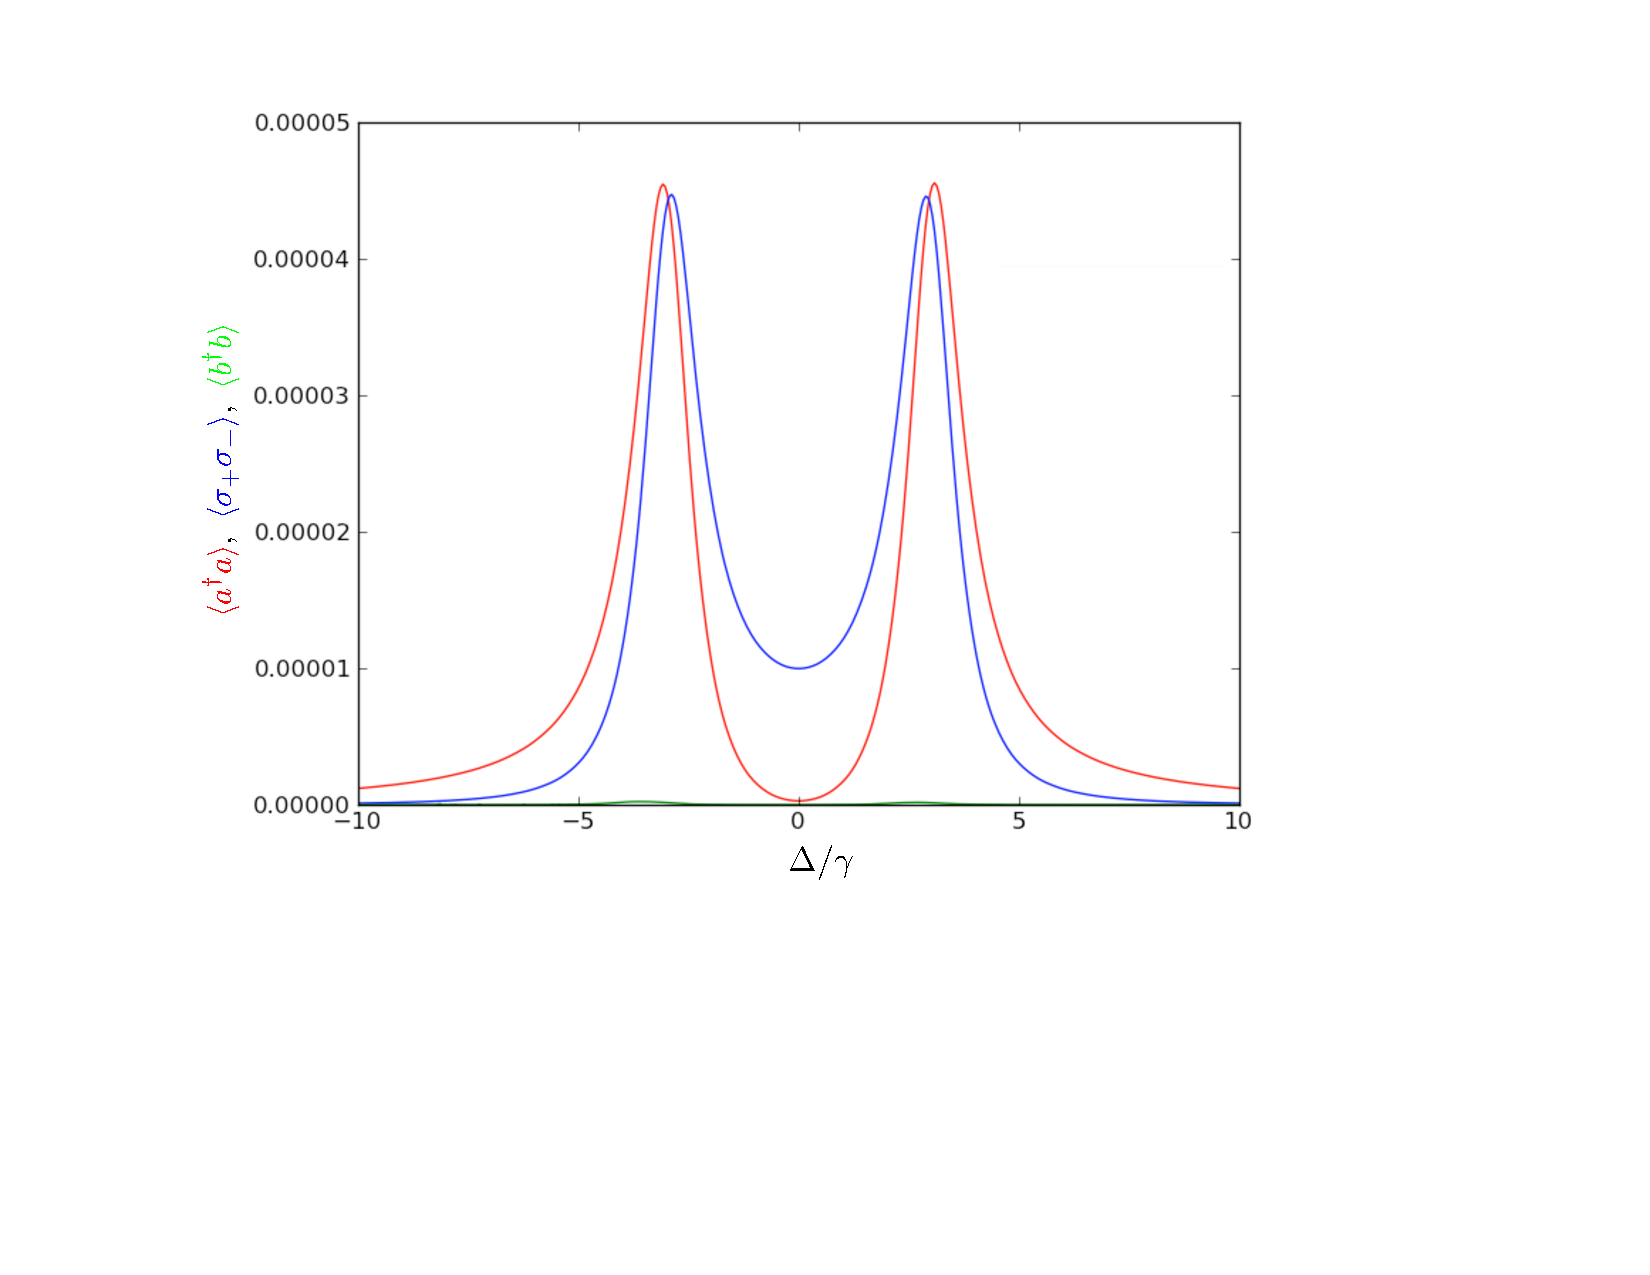
\includegraphics[width=0.474\textwidth]{Figures/5a_gM1_10}}
\qquad
\subfloat[\small{$g_M/\gamma = 1$}]{\label{fig5b}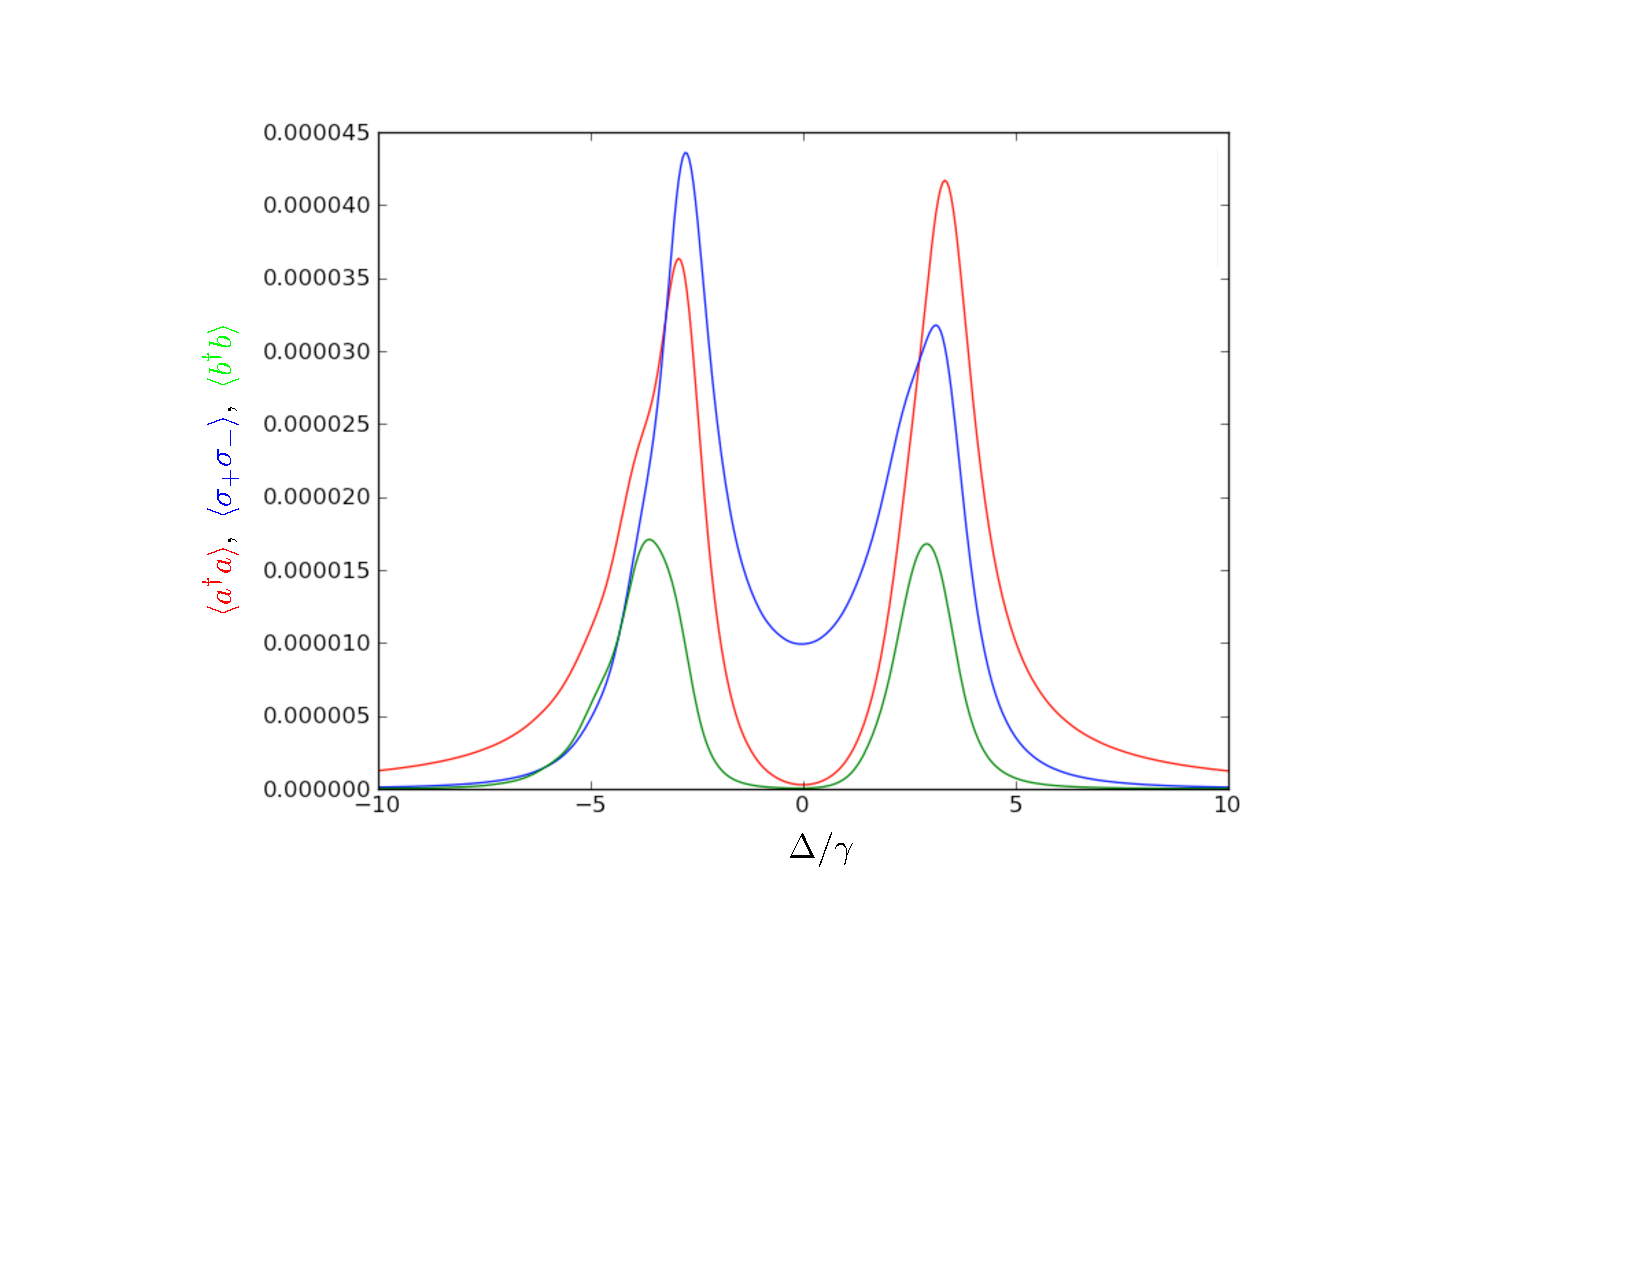
\includegraphics[width=0.474\textwidth]{Figures/5b_gM1}}
\\
\subfloat[\small{$g_M/\gamma = 3$}]{\label{fig5c}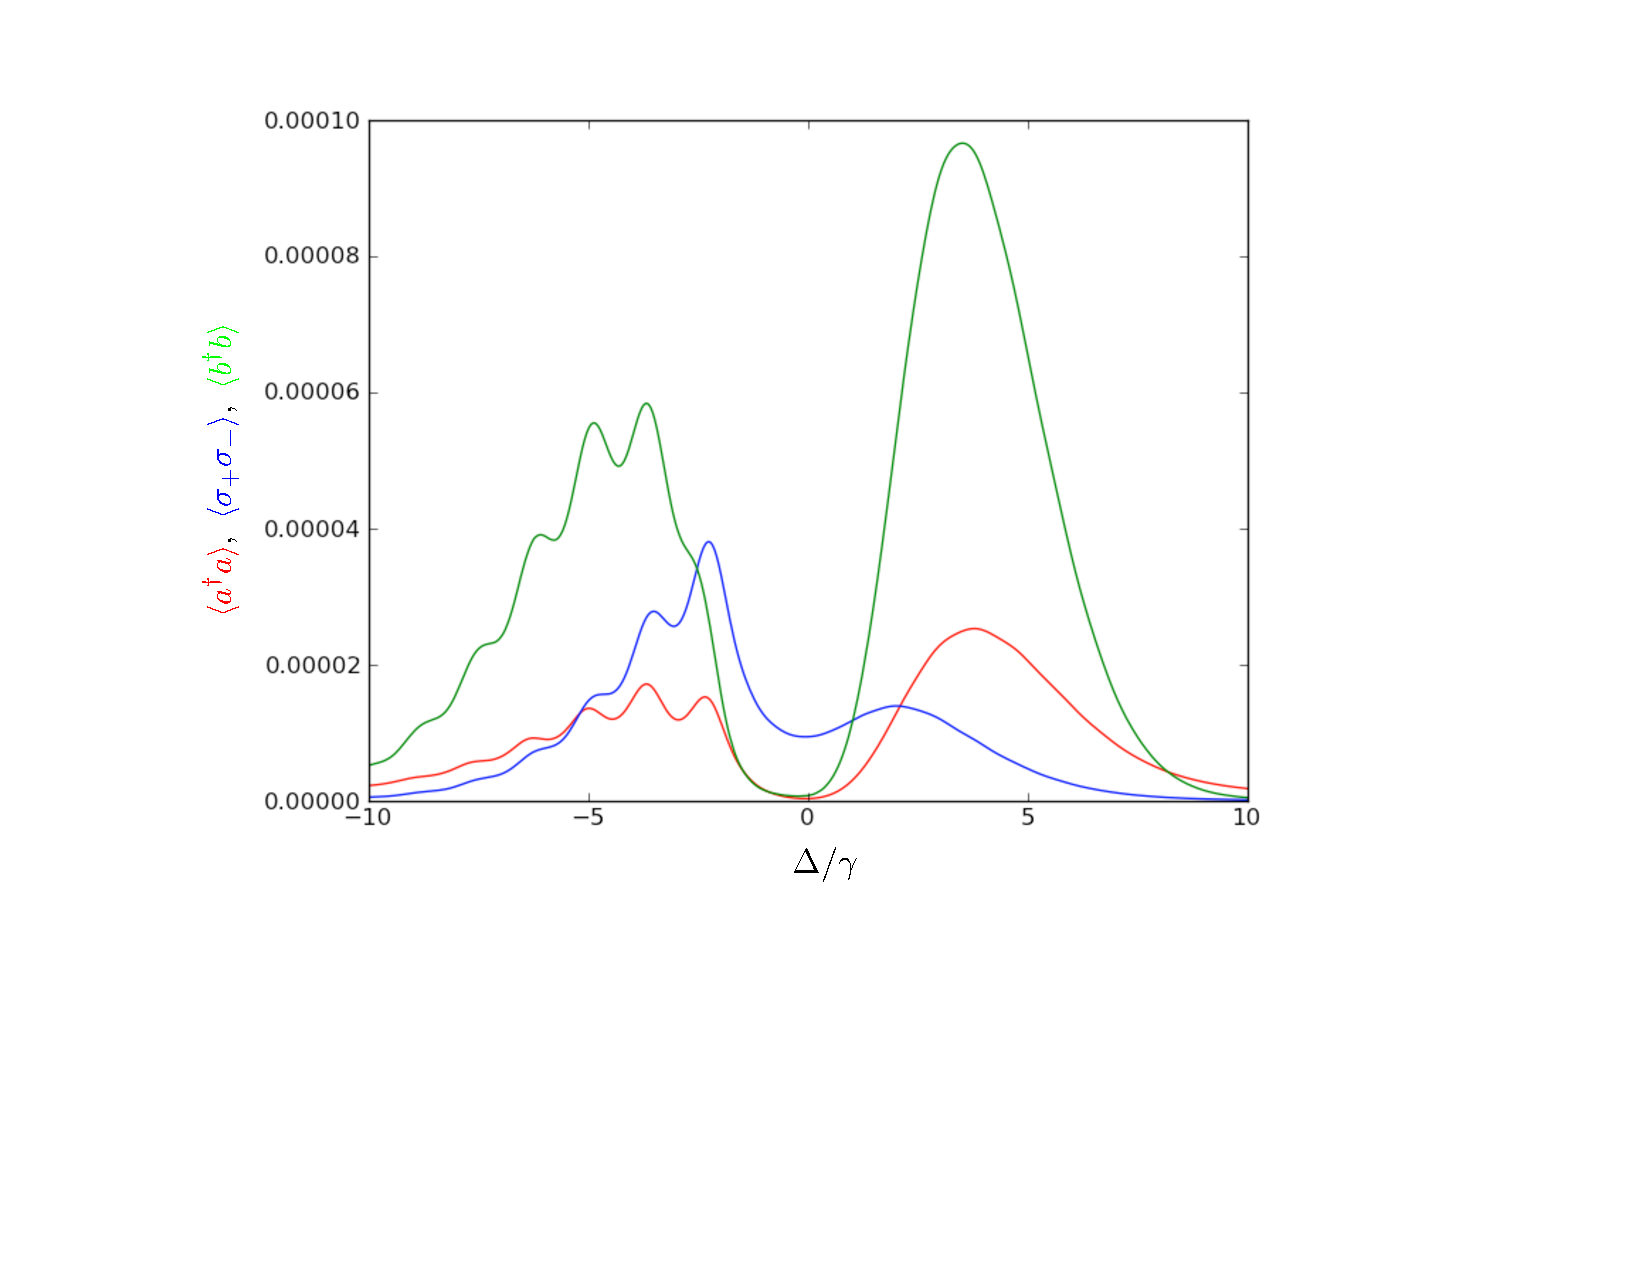
\includegraphics[width=0.474\textwidth]{Figures/5c_gM3}}
\qquad
\subfloat[\small{$g_M/\gamma = 5$}]{\label{fig5d}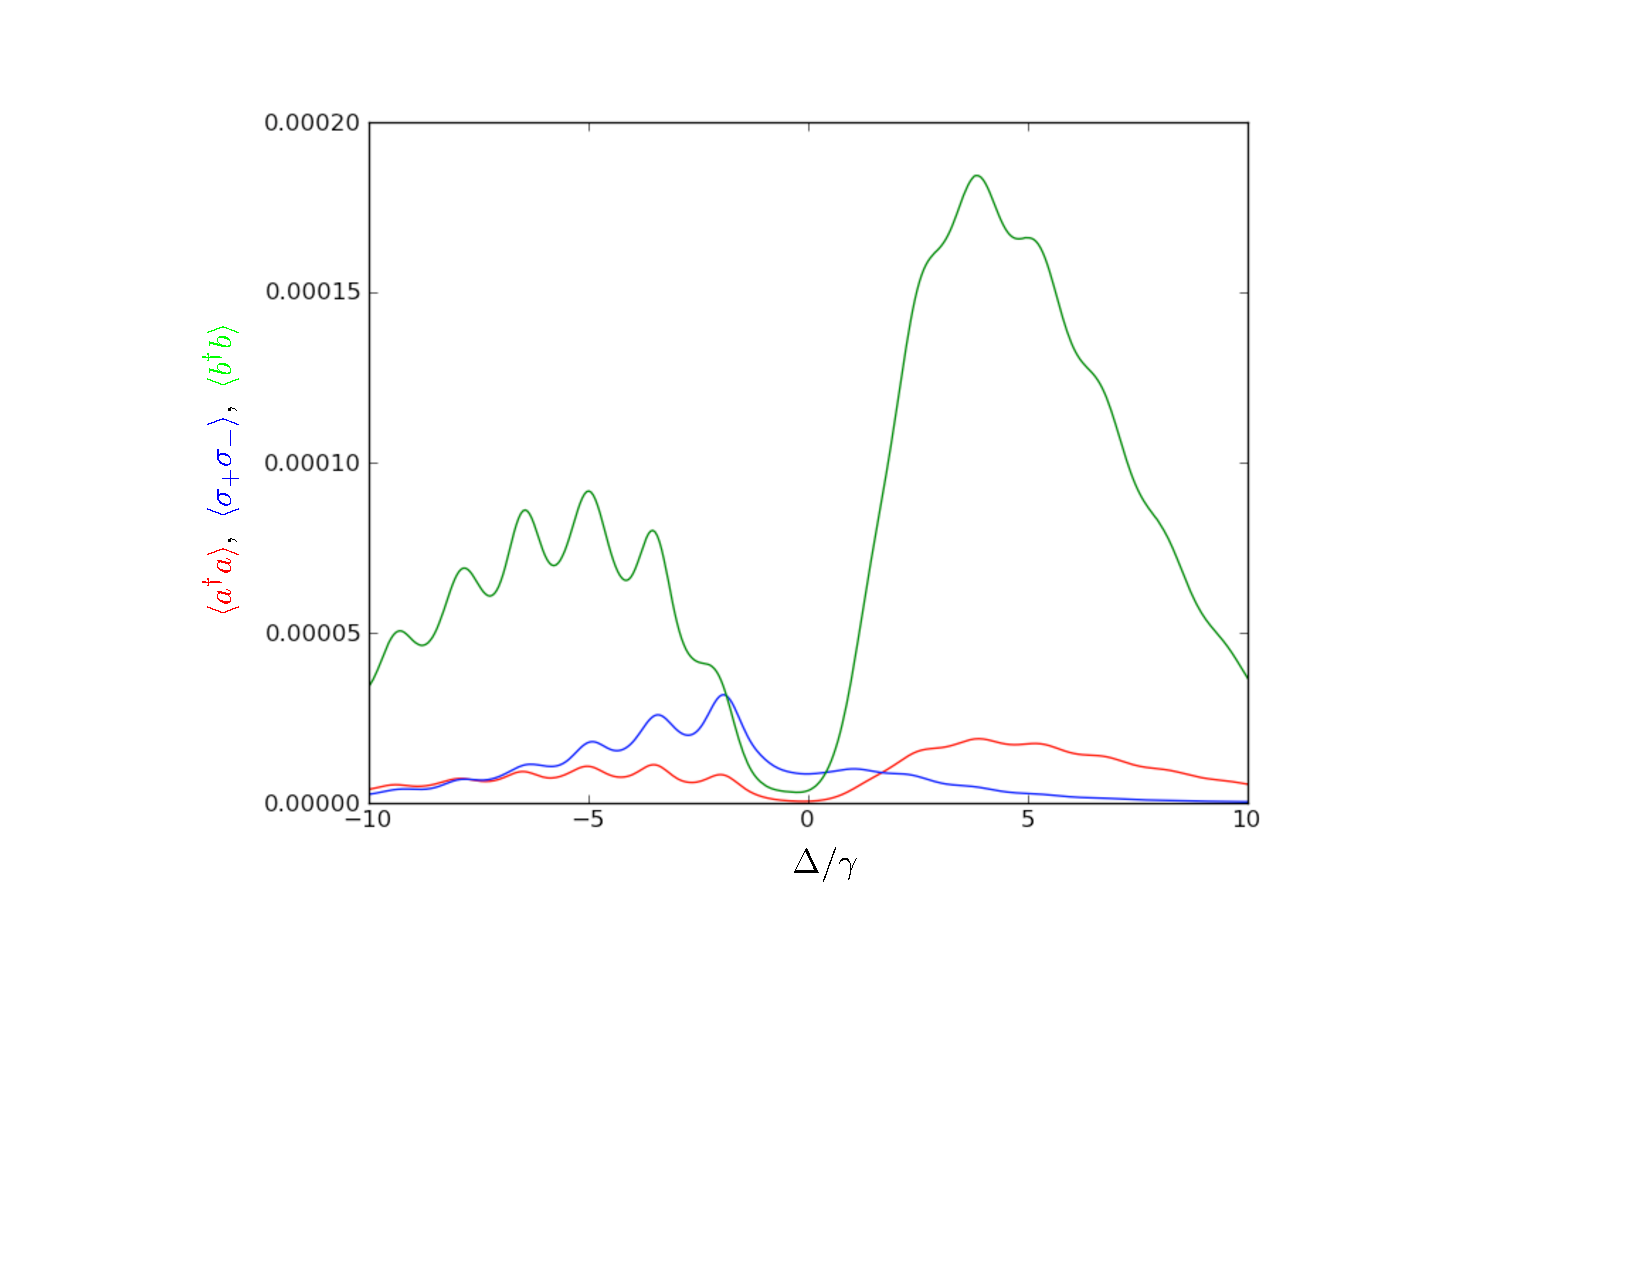
\includegraphics[width=0.474\textwidth]{Figures/5d_gM5}}
\caption[Probe spectra over a range of mechanical coupling rates]{\small{Probe spectra over a range of mechanical coupling rates with set optical coupling. Red traces indicate $\langle \adag a \rangle$, blue traces denote $\langle \splus\sminus \rangle$, and green traces indicate $\langle \bdag b \rangle$. The relevant parameters are $\gamma = \kappa = \omega_M = 1$, $Y/\gamma = 0.01$, and $g/\gamma = 3$. A maximum of 64 phonon excitations is allowed in the oscillator.}}
\label{fig5gM}
\end{figure}

\noindent Finally, we observe that as $g_M$ increases, a larger proportion of the total energy is stored in the form of phonon excitations.

In Fig.~\ref{fig6g}, we present a series of spectra where $g_M$ is constant and we calculate the relevant expectation values over a range of optical coupling values. Considering first Fig.~\ref{fig6a} where $g \ll g_M$, we see any signature of the atom's presence effectively vanishes, and we are in accordance with the cavity-oscillator model of \cite{girvin2011}. Setting $g/\gamma$ equal to unity, the signature vacuum Rabi doublet begins to become evident, but is still somewhat difficult to resolve due to the two peaks lying at $g \simeq \pm 1$. For $g > g_M$, the doublet is completely resolved, and it is clear that their structure is more complex than that of Figs.~\ref{fig5a}-\ref{fig5b}. It follows that as $g$ increases and surpasses $g_M$, a growing amount of the total energy is transferred from the oscillator to the atom-cavity subsystem.

\begin{figure}[htb]
\centering
\subfloat[\small{$g/\gamma = 0.1$}]{\label{fig6a}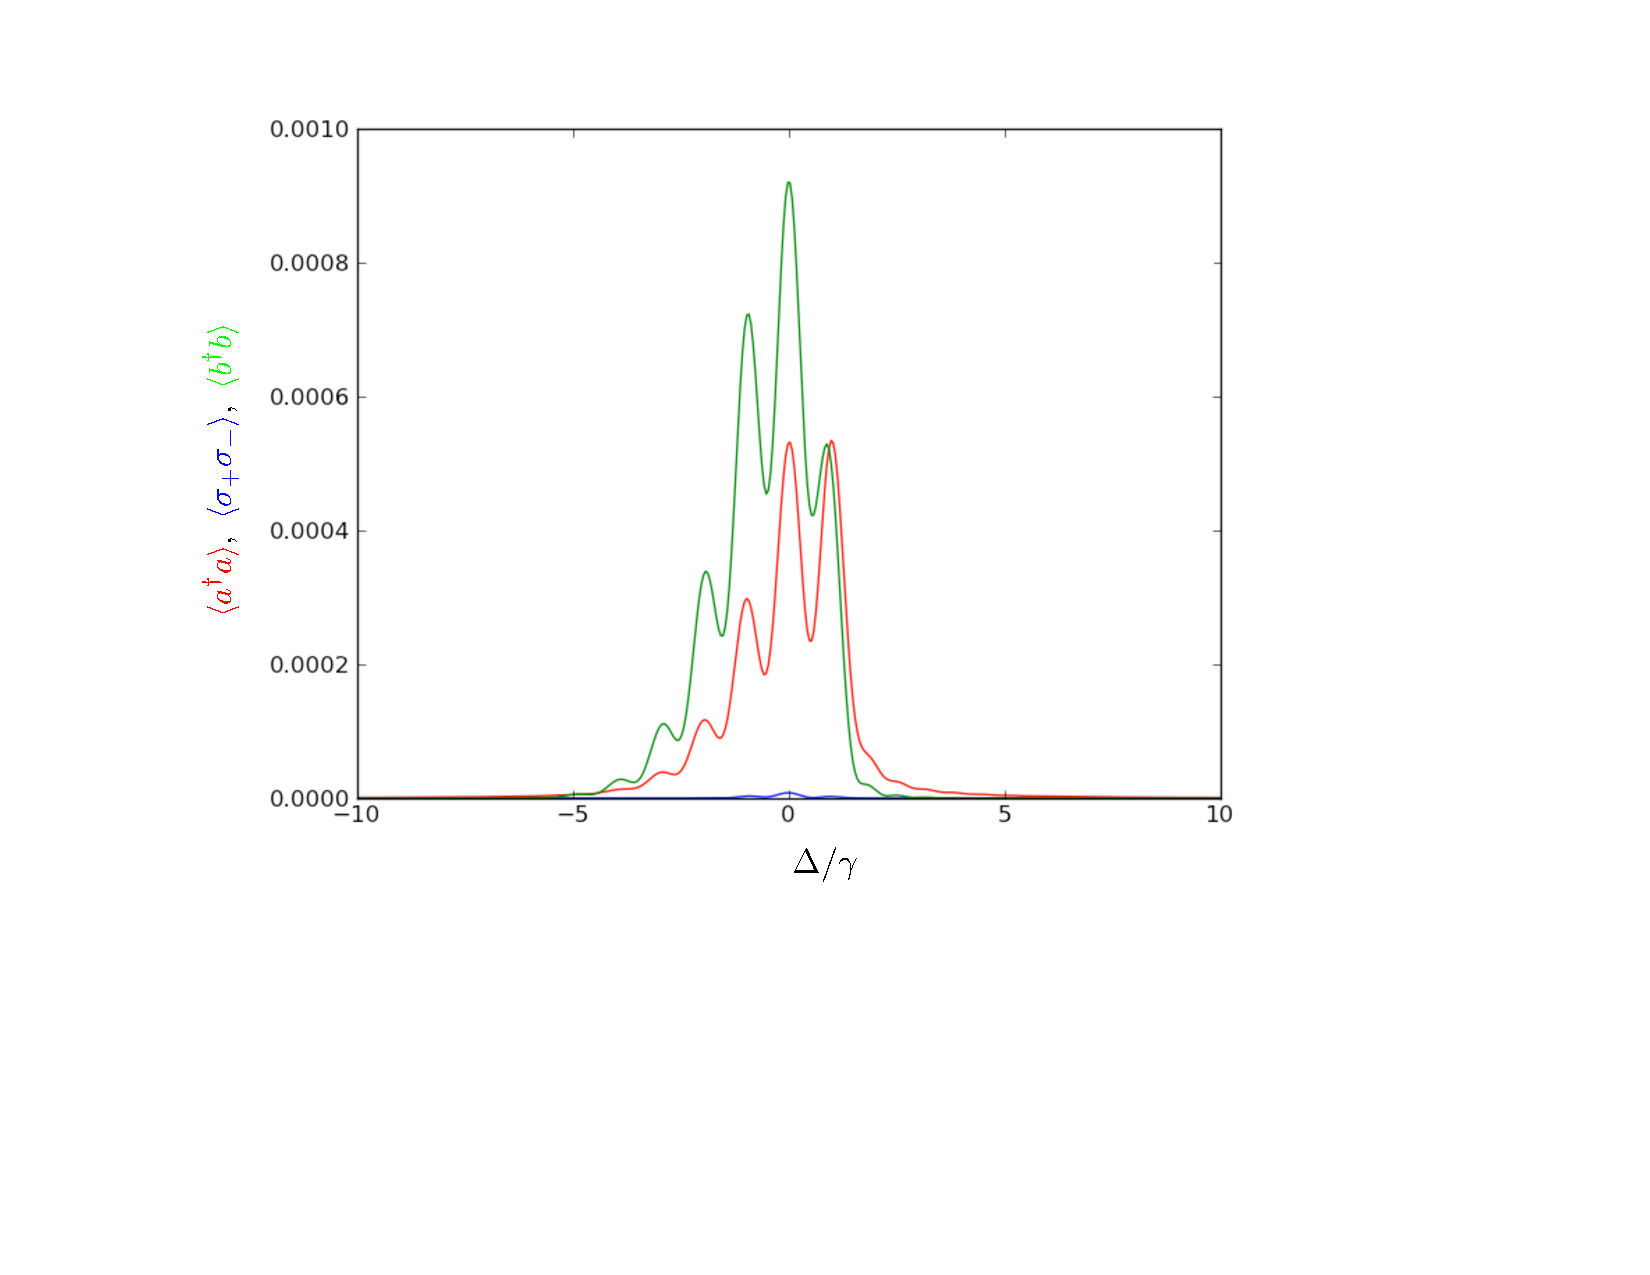
\includegraphics[width=0.474\textwidth]{Figures/6a_g1_10}}
\\
\subfloat[\small{$g/\gamma = 1$}]{\label{fig6b}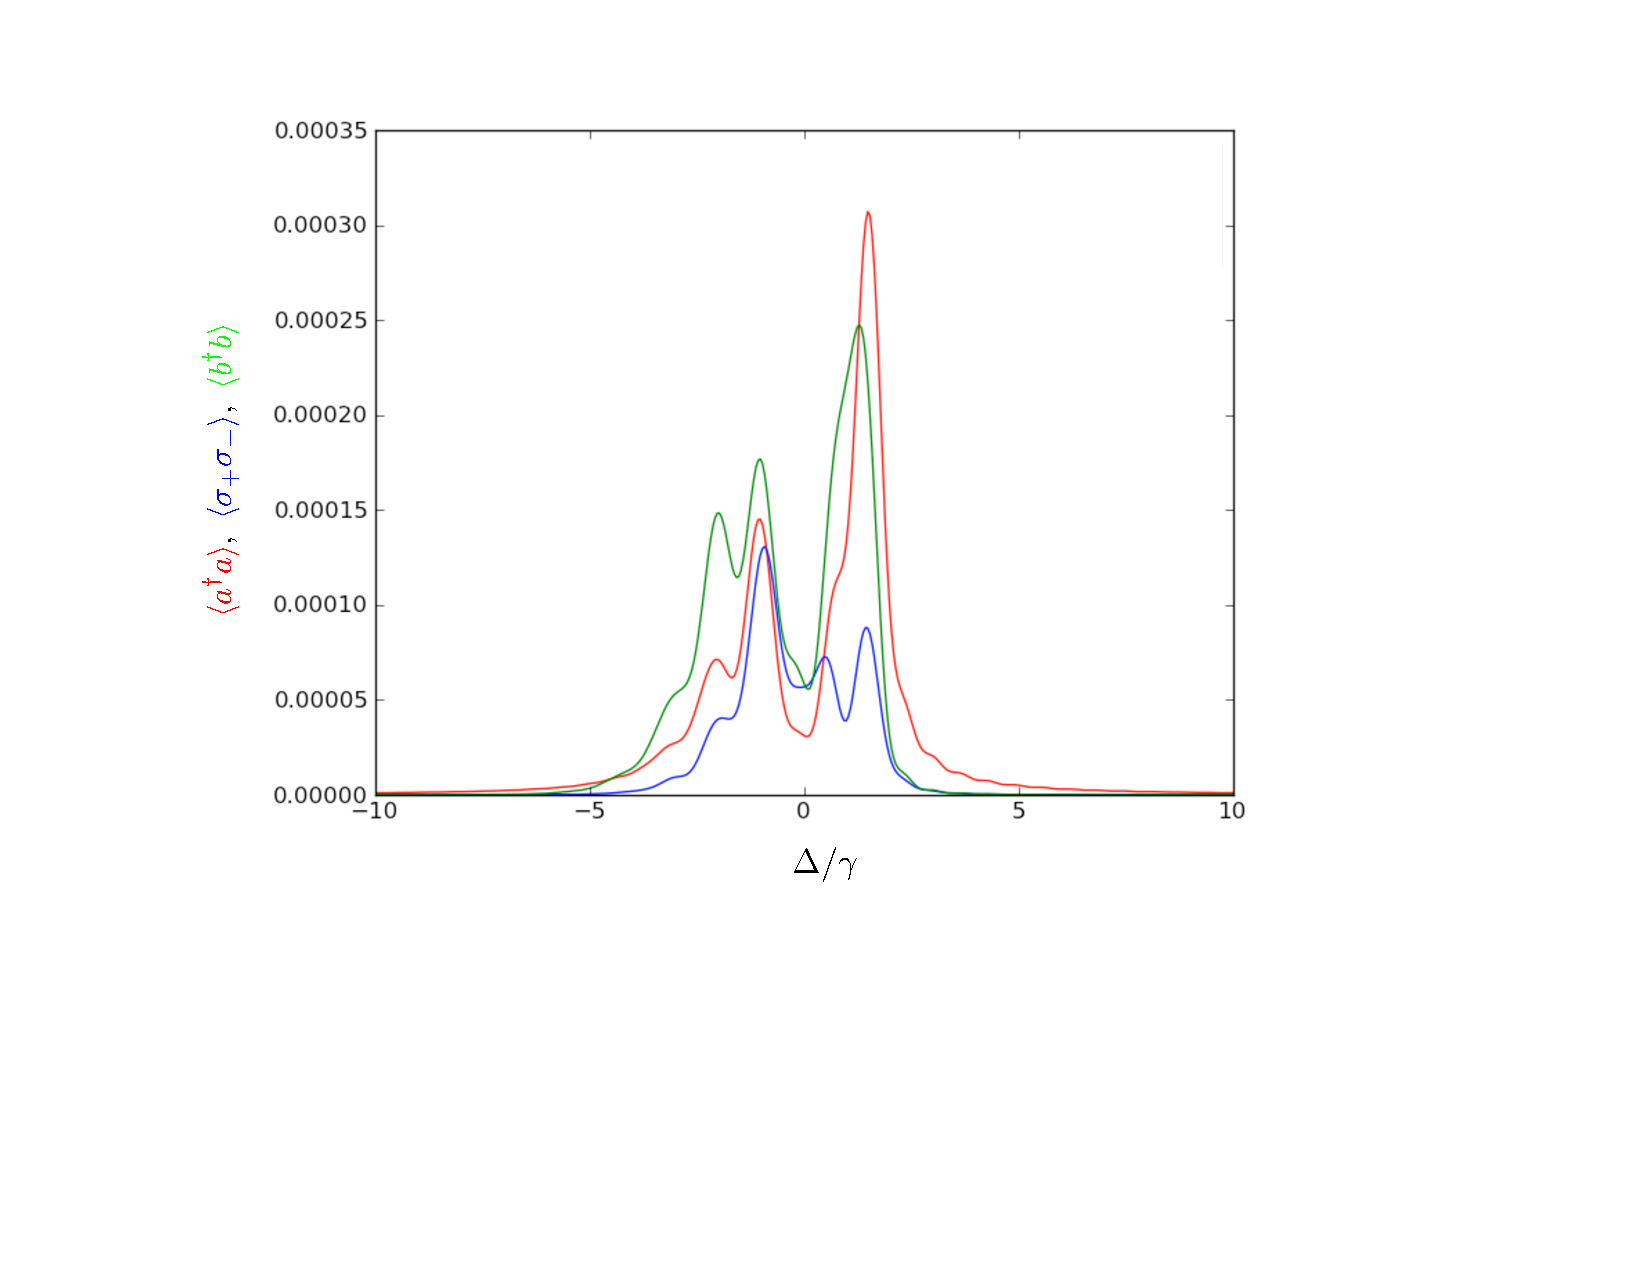
\includegraphics[width=0.474\textwidth]{Figures/6b_g1}}
\qquad
\subfloat[\small{$g/\gamma = 5$}]{\label{fig6c}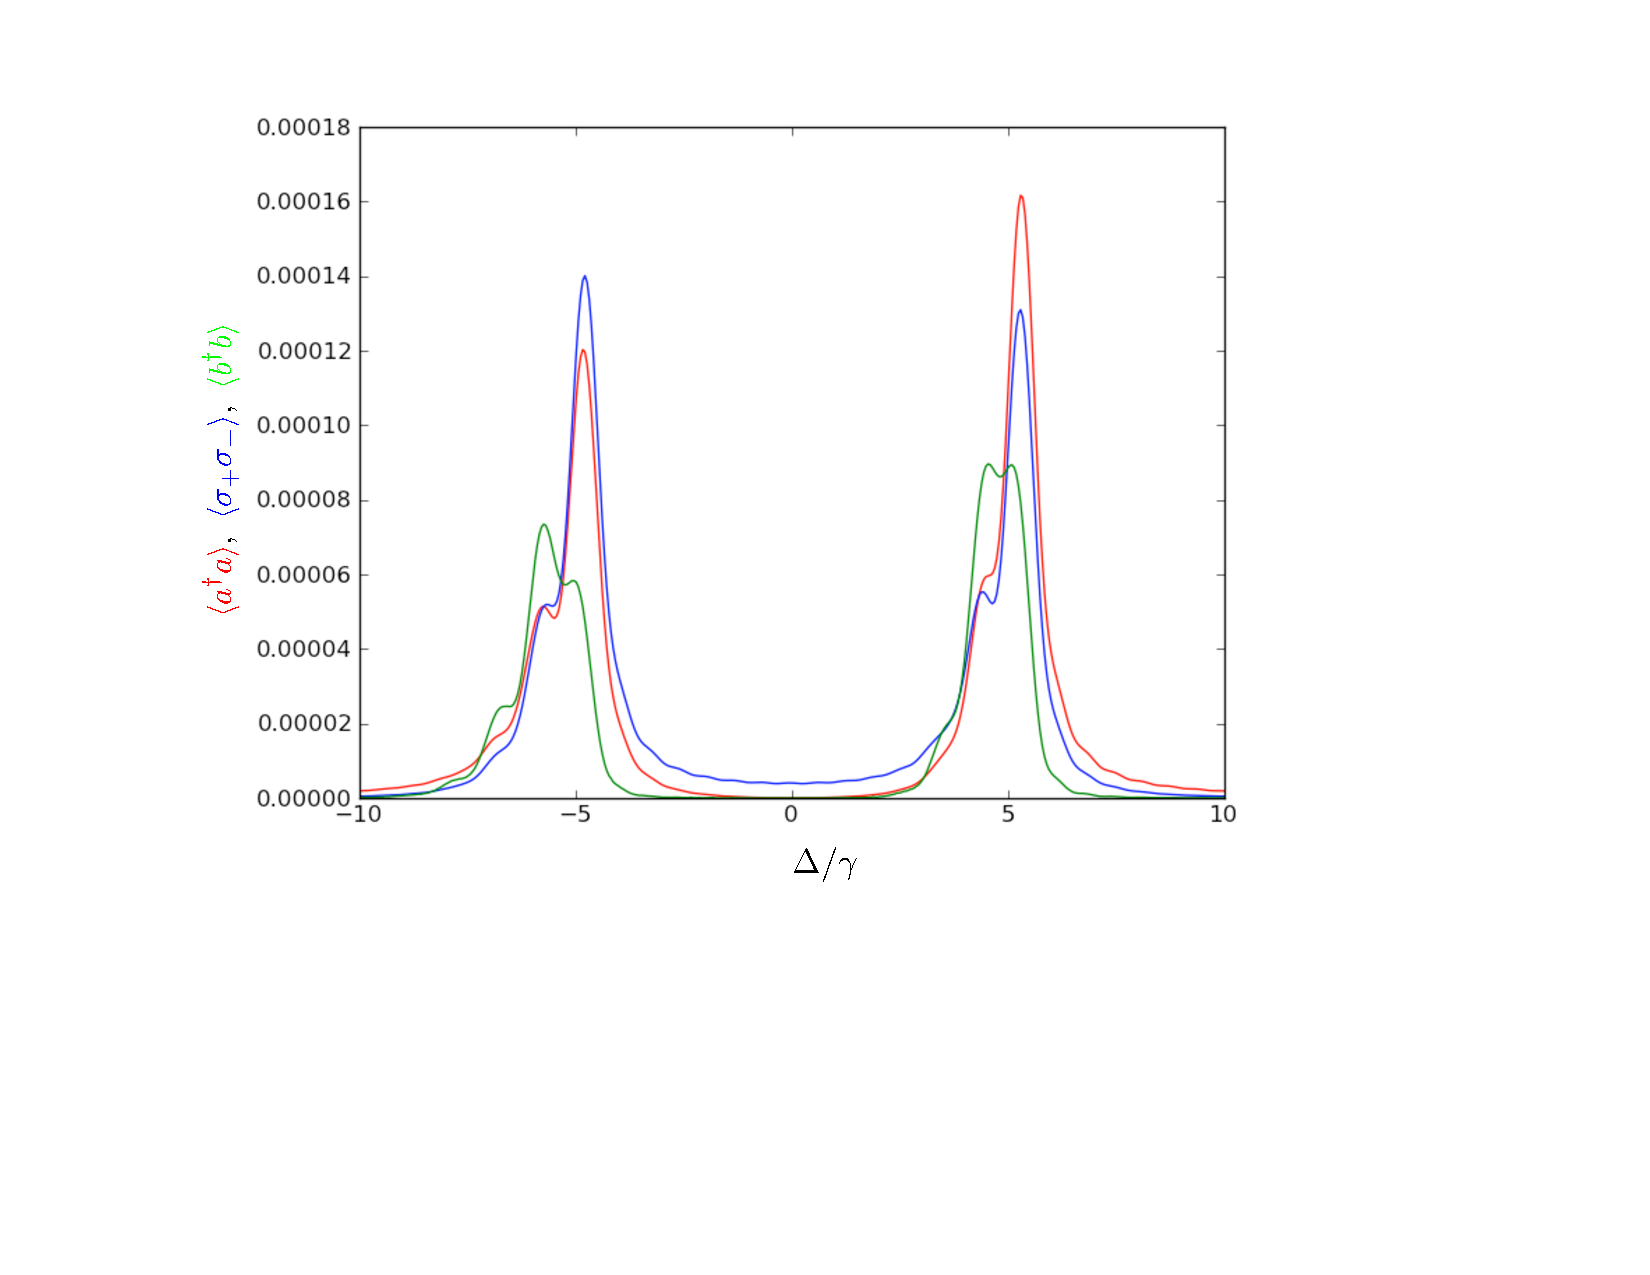
\includegraphics[width=0.474\textwidth]{Figures/6c_g5}}
\caption[Probe spectra over a range of optical coupling rates]{\small{Probe spectra over a range of optical coupling rates with set mechanical coupling. Red traces indicate $\langle \adag a \rangle$, blue traces denote $\langle \splus\sminus \rangle$, and green traces indicate $\langle \bdag b \rangle$. The relevant parameters are $\gamma = \omega_M = g_M = 1$, $\kappa/\gamma = 0.25$, and $Y/\gamma = 0.01$. A maximum of 64 phonon excitations is allowed in the oscillator.}}
\label{fig6g}
\end{figure}

In all of Section 4, on account of the weak incident field, we evaluate each trace with only a single trajectory due to the low probability for a jump to occur. Considering Figs.~\ref{fig5a}-\ref{fig6c}, this approximation is validated, as the highest mean value we see is $\langle \bdag b \rangle \sim 10^{-3}$ in Fig.~\ref{fig6a}, demonstrating that all three subsystems occupy their respective ground states. As a final note, we remark that all values in Figs.~\ref{fig5gM} and \ref{fig6g} are steady-state expectation values, reached after ten spontaneous emission lifetimes.

\section{Photon Statistics}
In the context of cavity QED, photon statistics play a valuable role in many aspects of study. Measurement of the second-order correlation function of a transmitted electromagnetic field allow experimenters to deduce the nonclassical nature of the light source \cite{leach2003}. Indeed, such measurements also provide evidence that certain atomic and cavity quantum states are capable of being ``frozen'' in their time evolution, only to be restarted at a later time as if no such interruption occurred \cite{leach2003}. New types of correlation functions are also being developed, such as $h_{\theta}(\tau)$ by Carmichael \emph{et. al.}, which measures the correlation between a photon detection and conditional field fluctuations, bringing to light the junction between the particle and wave natures of light \cite{leach2003}.

Our investigation of photon statistics begins with consideration of the normalized, steady-state second-order correlation function $g^{(2)}(0)$, specifically the field-field auto-correlation and atom-field cross-correlation. We follow the approach of \cite{brecha1999} in the respective calculations,
%
\begin{align} g^{(2)}_{aa}(0) &= \frac{\evalue{a^{\dag 2} a^2}}{\evalue{\adag a}^2}, \label{eq4.1} \\[5pt]
g^{(2)}_{a\gamma}(0) &= \frac{\evalue{\adag a \, \splus\sminus}}{\evalue{\adag a} \evalue{\splus\sminus}}. \label{eq4.2} \end{align}
%
Typically, $g^{(2)}(0)$ is plotted as a function of parameters such as cavity linewidth $\kappa$ or detuning $\Delta$; in a multiatom ensemble case, the correlation function will be plotted as a function of atomic number \cite{brecha1999}. In the case of cOM, we plot $g^{(2)}(0)$ as a function of mechanical coupling $g_M$. Note that we include mechanical damping with $\kappa_M > 0$, and determine \eqref{eq4.1} and \eqref{eq4.2} on resonance, $\Delta = 0$.

We pause now to justify our choice in Fig.~\ref{fig7g20} for the optical coupling constant $g/\gamma = 1/\sqrt{2}$. Following the approach of \cite{howard1991}, the analytical result for the second-order correlation function at $\tau = 0$ is
%
\be g^{(2)}(0) = 1 + \frac{\Delta\alpha}{\alpha}, \label{eq4.3} \ee
%
where
%
\be \frac{\Delta\alpha}{\alpha} = -2C'_1 \left( \frac{2C}{1 + 2C - 2C'_1} \right), \label{eq4.4} \ee
%
and
%
\be C = \frac{g^2}{\gamma\kappa}, \quad C'_1 = \frac{C}{1 + (\gamma/2\kappa)}. \label{eq4.5} \ee
%
\newpage
\begin{figure}[htb]
\begin{center}
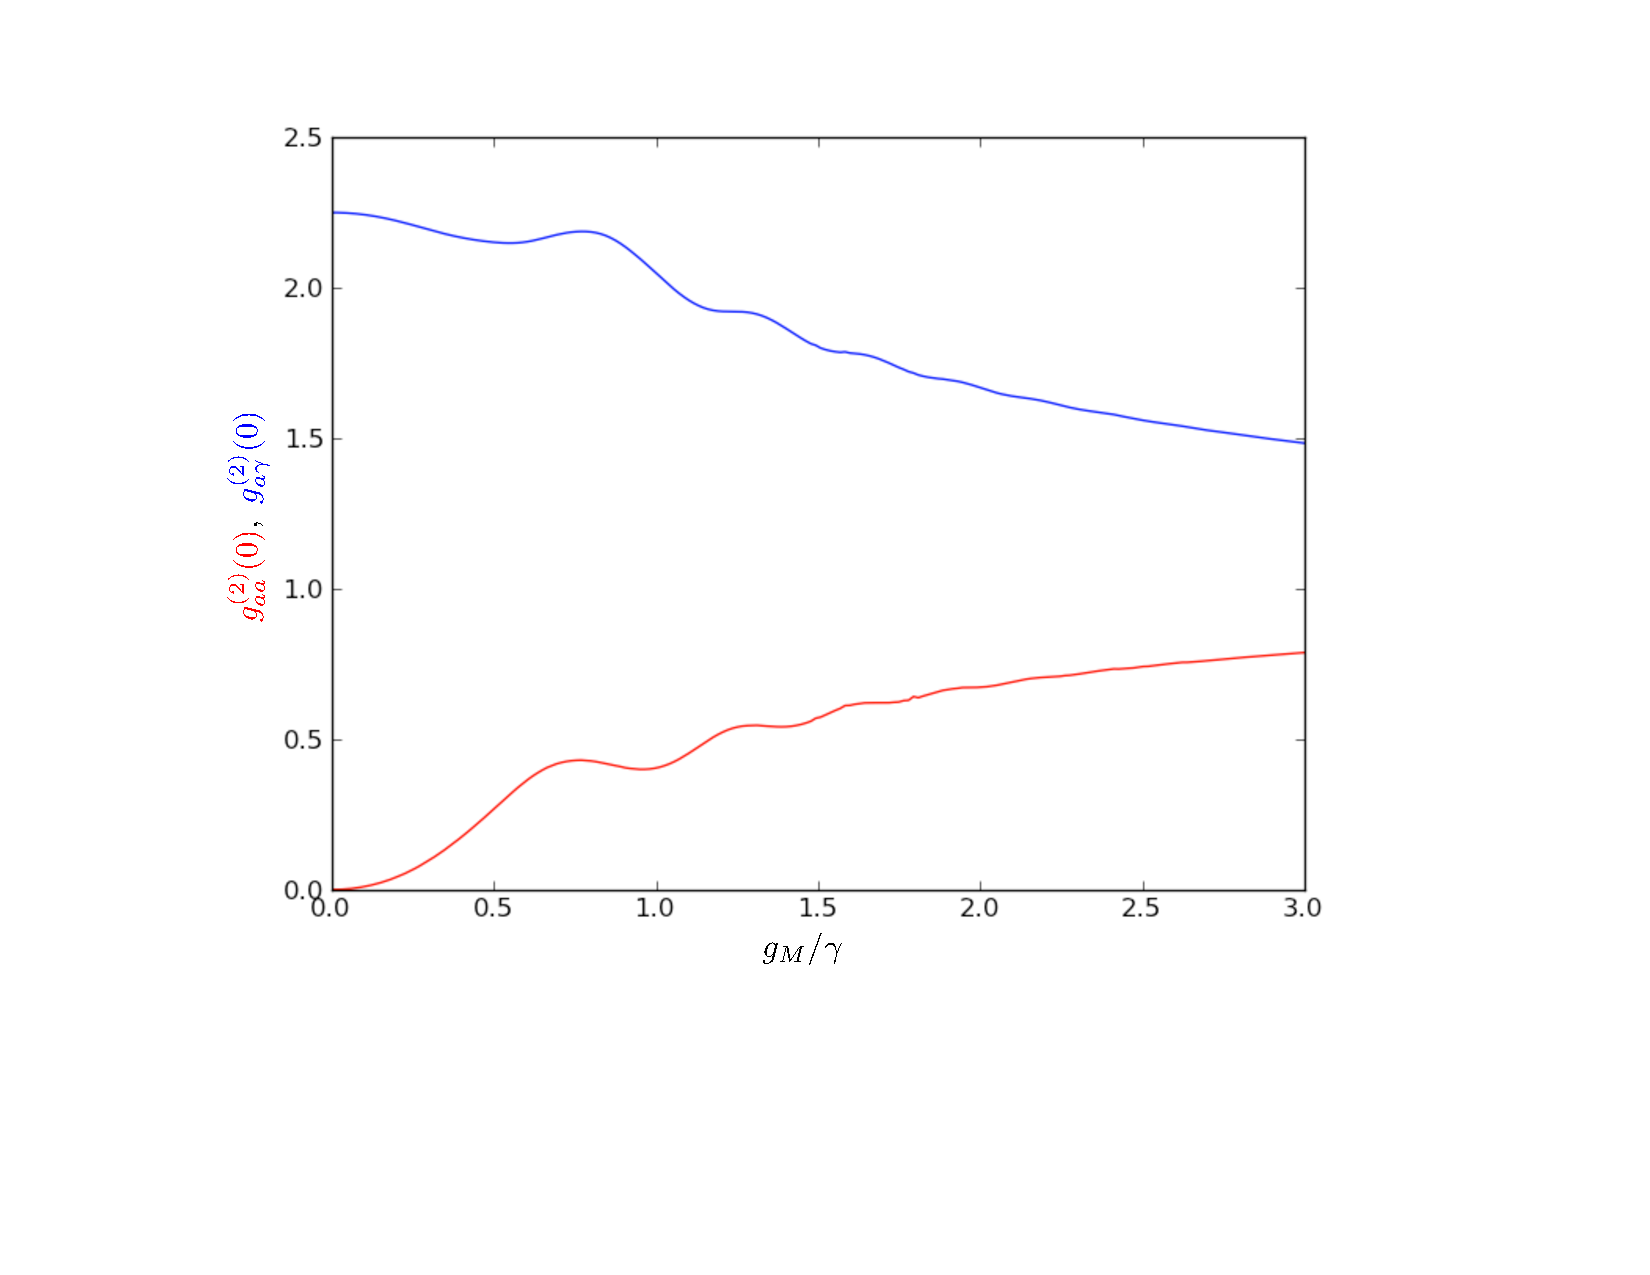
\includegraphics[width=0.85\textwidth]{Figures/7g20}
\caption[A plot of $g^{(2)}(0)$ in the steady state as a function of $g_M$]{\small{A plot of the second-order correlation function $g^{(2)}(0)$, as a function of mechanical coupling $g_M$, after allowing $10\tau_0$ to reach the steady state. The red trace denotes the field-field auto-correlation, while the blue trace indicates the atom-field cross-correlation. The relevant parameters are $\gamma = \omega_M = 1$, $Y/\gamma = 0.01$, $\kappa/\gamma = 0.5$, $g/\gamma = 1/\sqrt{2}$, and $\kappa_M/\gamma = 0.1$. The maximal atom-cavity excitation number is raised to 3, while the phonon excitation limit is raised to 128.}}
\label{fig7g20}
\end{center}
\end{figure}

\noindent The parameter $C$ in \eqref{eq4.5} appears frequently in cQED and is known as the cooperativity. Our objective now is to choose a set of parameters $\left\{ \gamma, \, \kappa, \, g \right\}$ such that the field-field auto-correlation demonstrates perfect photon antibunching, i.e. $g^{(2)}(0) = 0$, in the limit $g_M \to 0$. Using the values $\gamma = 1$ and $\kappa = \gamma/2 = 0.5$, we see from \eqref{eq4.5} that $C'_1 = C/2$ such that \eqref{eq4.4} reduces to
%
\be \frac{\Delta\alpha}{\alpha} = -C \left( \frac{2C}{1 + C} \right), \label{eq4.6} \ee
%
and because $C = 2g^2$ we find
%
\be \frac{\Delta\alpha}{\alpha} = -2g^2 \left( \frac{4g^2}{1 + 2g^2} \right) = -1, \label{eq4.7} \ee
%
where the value of $-1$ is chosen in order to satisfy $g^{(2)}(0) = 0$ in \eqref{eq4.3}. We obtain from \eqref{eq4.7}
%
\be -8g^4 + 2g^2 + 1 = 0, \label{eq4.8} \ee
%
a quadratic equation in $g^2$; defining $x \equiv g^2$ and using the quadratic formula we obtain $x = (1/8) \pm (3/8)$. The negative root of $x$ is discarded as it ultimately yields an unphysical (imaginary) value for $g$. The optimal value for the coupling constant must then be $g_{\text{opt}} = \sqrt{x} = \sqrt{1/2}$, validating our choice in Fig.~\ref{fig7g20}.

We observe in the traces of $g^{(2)}(0)$ that the field-field and atom-field correlations are respectively antibunched and bunched without any optomechanical coupling present. As the oscillator coupling is increased, both correlations approach a value of unity, indicating they come closer to obeying Poissonian photon statistics. This is a similar result to the influence of parameters $N$ (atom number) and $\Delta$ on the correlations in \cite{brecha1999}.

Continuing with our discussion of photon statistics, we generalize to a calculation of the time-varying, normalized, second-order correlation function $g^{(2)}(\tau)$. We again calculate the field-field auto-correlation and atom-field cross-correlation, plus we add the oscillator-field cross-correlation. Rather than referring to mathematical formalism as with $g^{(2)}(0)$, we numerically evaluate the former function, again using the technique of quantum trajectories and the \texttt{mcsolve} function of QuTiP.

We see from Figs.~\ref{fig8a} and \ref{fig8b} that the field-field and atom-field correlations undergo identical time evolution, starting in a bunched state and then oscillating anharmonically about unity. The oscillator-field correlations begin in a highly bunched state, $g^{(2)}(\tau) \gg 1$, and within a time period of $5\tau_0$ have decayed and oscillate about unity. Both statements are somewhat similar to the results of \cite{brecha1999}.

In order to calculate the $g^{(2)}(\tau)$, we first allow the initial ground state $\ket{\psi(0)}$ to evolve in time for $20\tau_0$ under the Hamiltonian of \eqref{eq2.107}, with $\Delta = 0$, to the steady state $\ket{\psi(20\tau_0)}_{ss}$. One of the three possible jump operators is then applied to the latter steady state, and the associated expectation value after another $20\tau_0$ due to the final state is used to determine the respective correlation functions. Finally, in order to normalize, the value is divided by the steady-state mean photon number under $\ket{\psi(20\tau_0)}_{ss}$ for each time step. To better illustrate the process, we denote the three final states after a jump and reaching the steady state as
%
\be \ket{\psi_a}_{ss} = \hat{\Upsilon}_{20} \, a \ket{\psi(20\tau_0)}_{ss}, \quad \ket{\psi_{\gamma}}_{ss} = \hat{\Upsilon}_{20} \, \sminus \ket{\psi(20\tau_0)}_{ss}, \quad \ket{\psi_b}_{ss} = \hat{\Upsilon}_{20} \, b \ket{\psi(20\tau_0)}_{ss}, \label{eq4.9} \ee
%
\newpage
\begin{figure}[htb]
\centering
\subfloat[\small{field-field}]{\label{fig8a}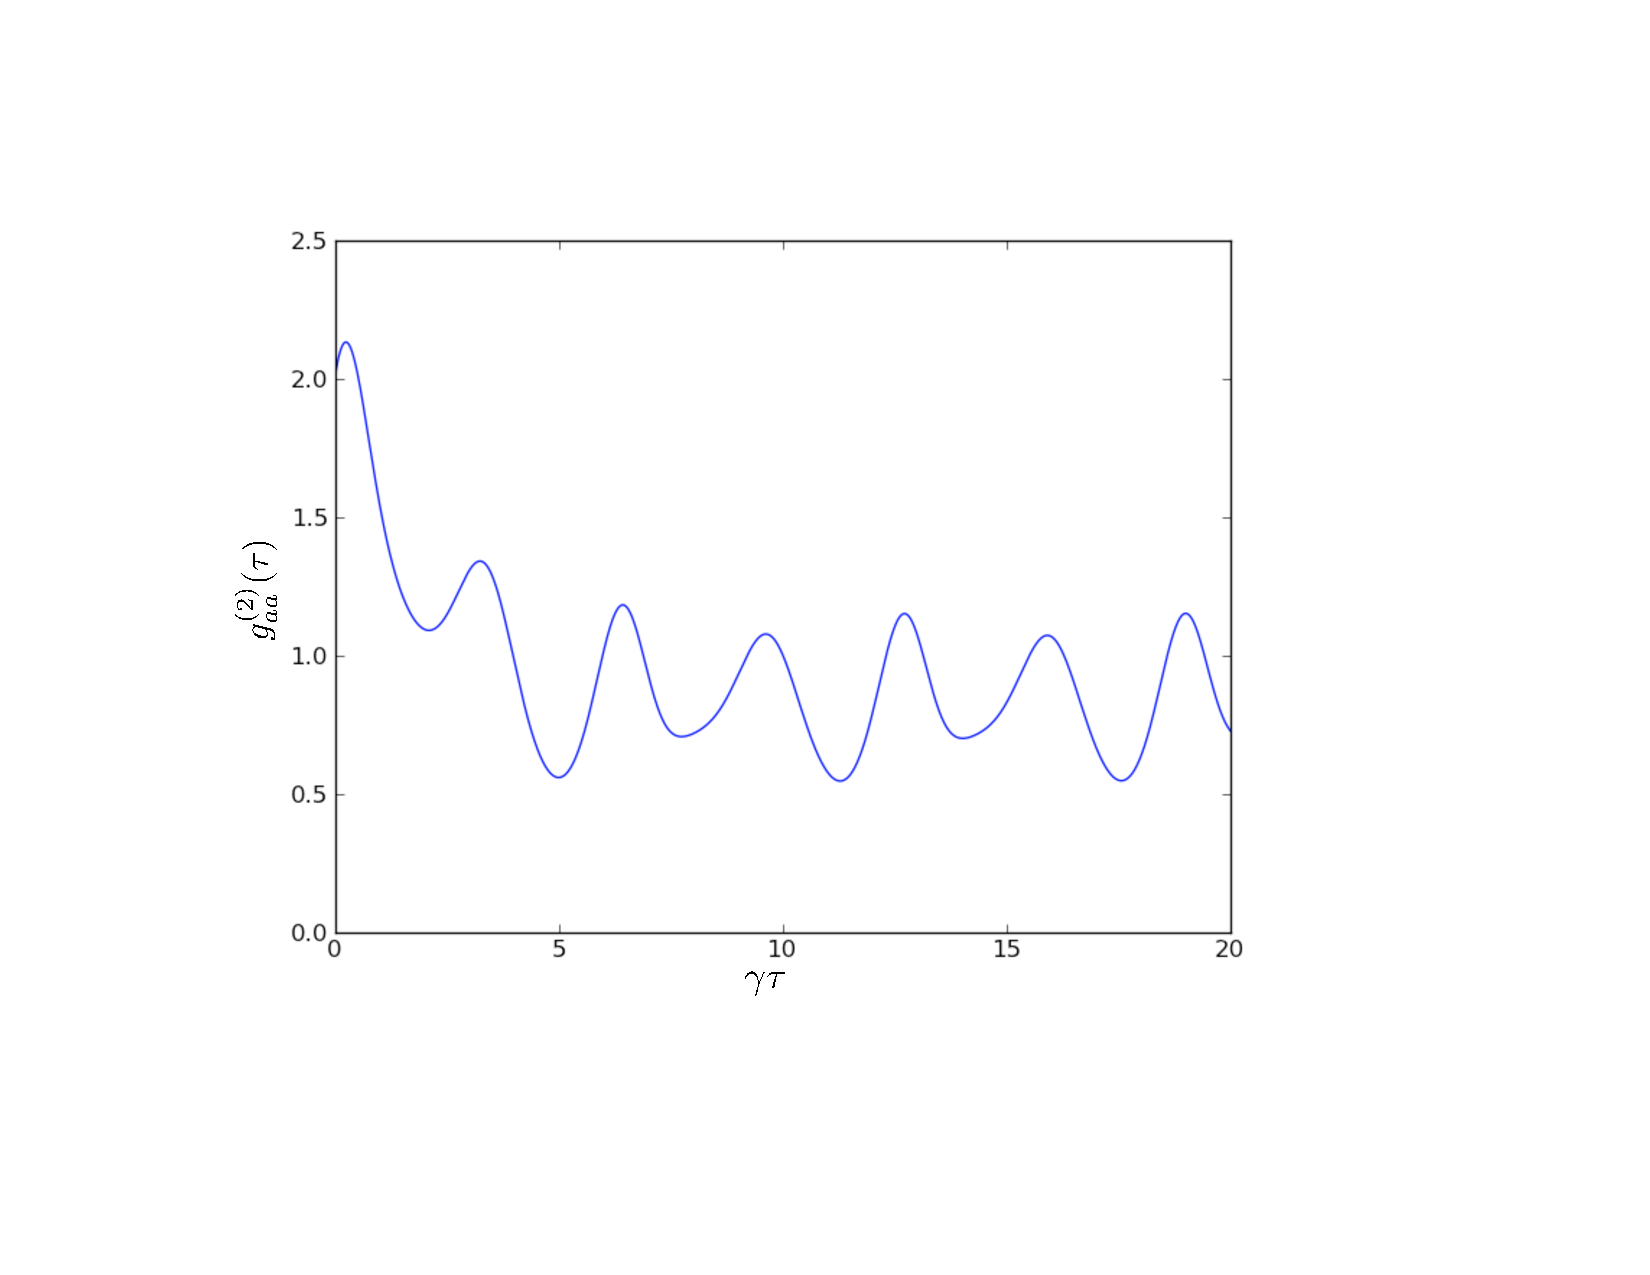
\includegraphics[width=0.474\textwidth]{Figures/8a_g2aatau}}
\qquad
\subfloat[\small{atom-field}]{\label{fig8b}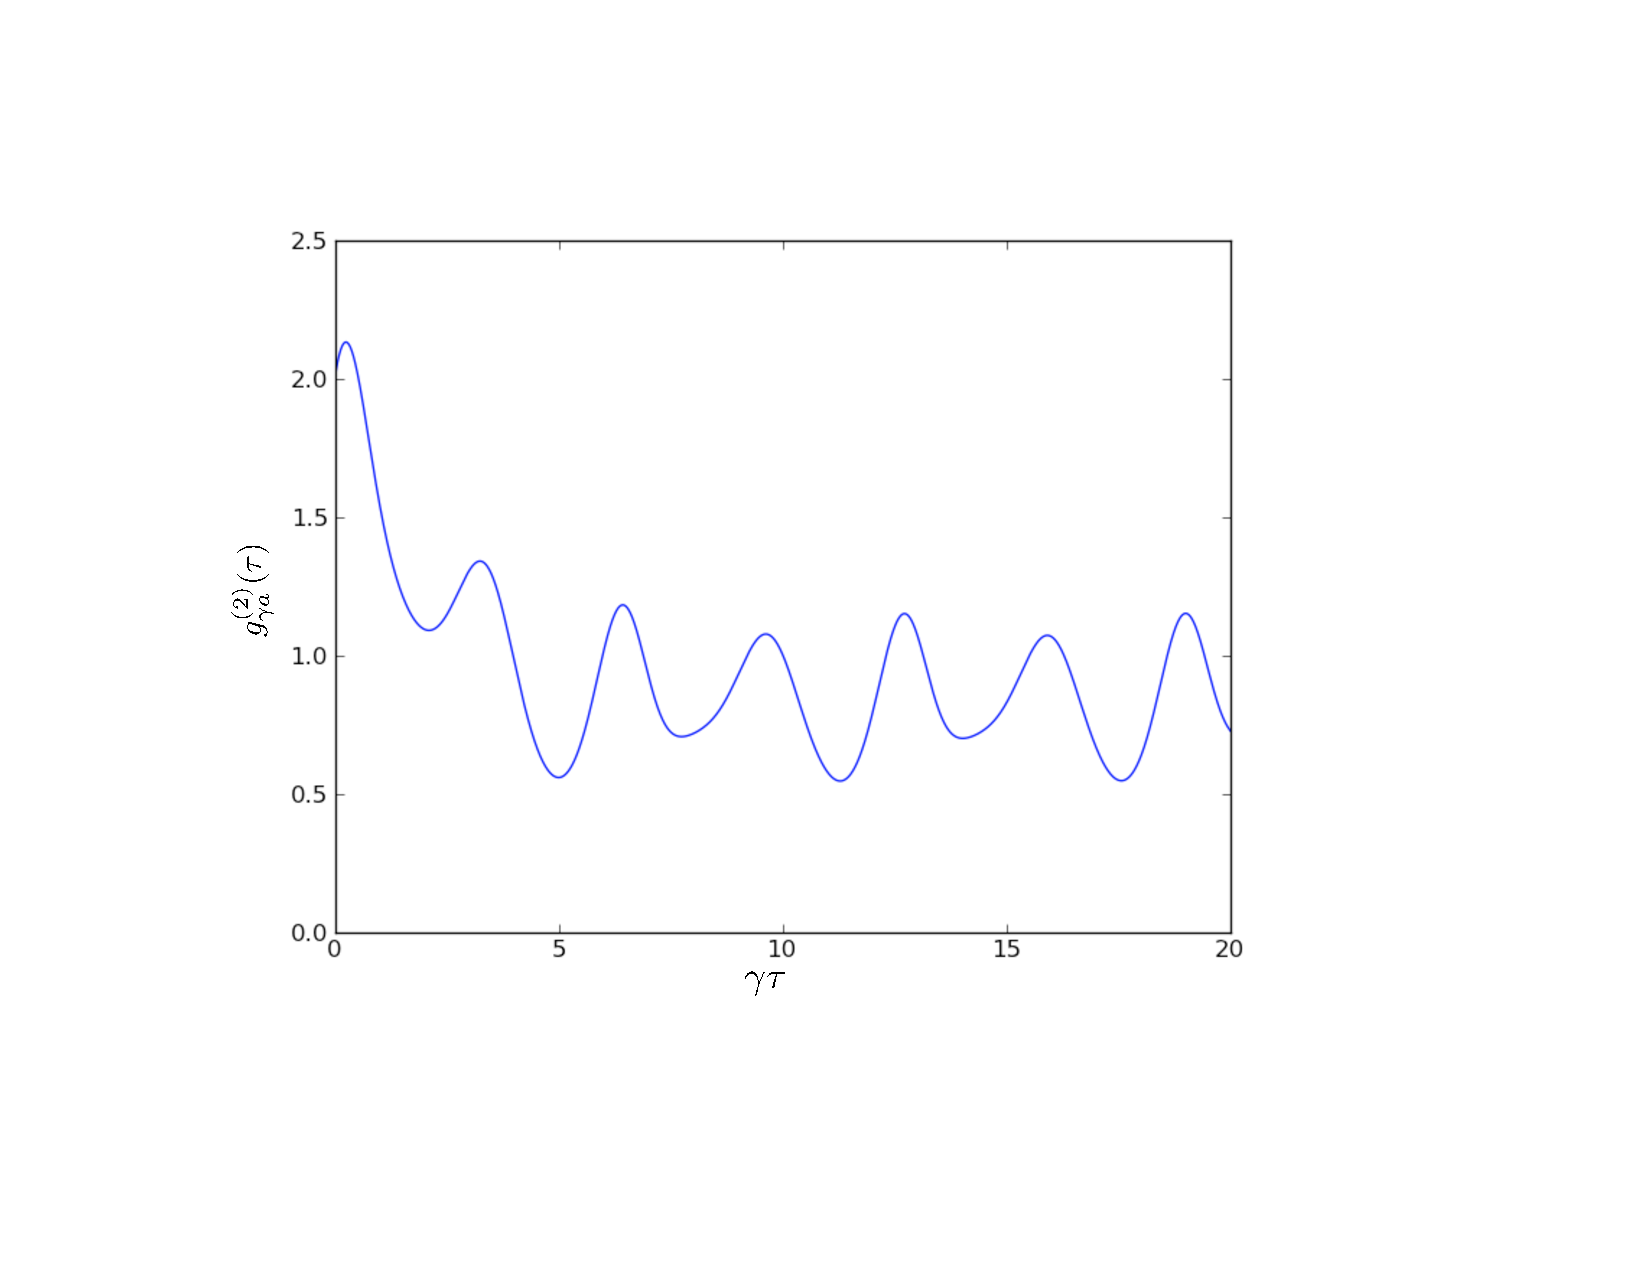
\includegraphics[width=0.474\textwidth]{Figures/8b_g2gatau}}
\\
\subfloat[\small{oscillator-field}]{\label{fig8c}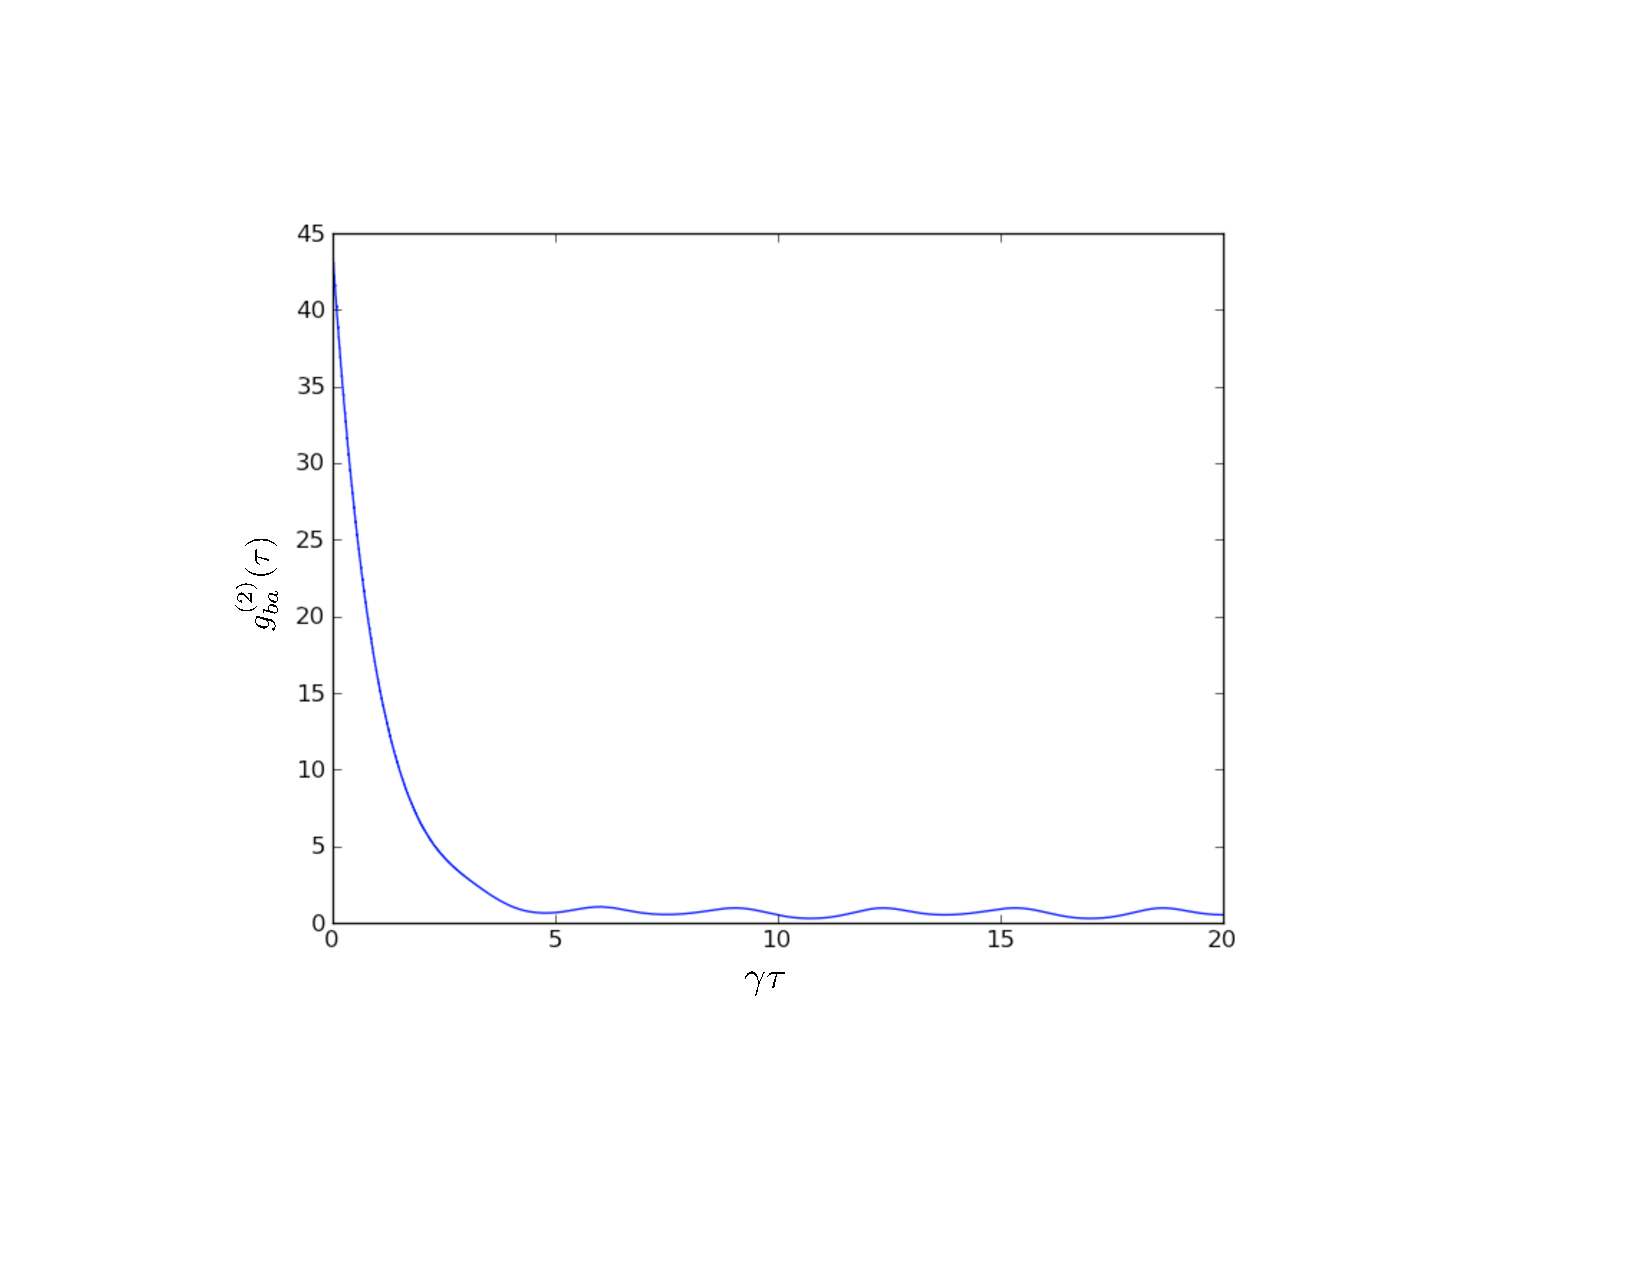
\includegraphics[width=0.474\textwidth]{Figures/8c_g2batau}}
\caption[Plots of $g^{(2)}(\tau)$ ]{\small{Plots of $g^{(2)}(\tau)$ over time. All steady-state expectation values are determined after $20\tau_0$. The relevant parameters are $\gamma = \omega_M = g_M = 1$, $\kappa/\gamma = 0.5$, $g/\gamma = 1/\sqrt{2}$, $\kappa_M/\gamma = 0.1$, and $Y/\gamma = 0.01$. As in Fig.~\ref{fig7g20}, we allow a maximum of 3 photon and 128 phonon excitations.}}
\label{fig8g2tau}
\end{figure}

\noindent where $\hat{\Upsilon}_{20}$ is an operator denoting another period of $20\tau_0$ of free evolution under the resonant $H$. The three correlation functions are then calculated by
%
\begin{align} g^{(2)}_{aa}(\tau) &= \frac{\langle \adag a \rangle_{a,ss}}{\langle \adag a \rangle_{ss}}, \label{eq4.10} \\[5pt]
g^{(2)}_{\gamma a}(\tau) &= \frac{\langle \splus\sminus \rangle_{\gamma,ss}}{\langle \adag a \rangle_{ss}}, \label{eq4.11} \\[5pt]
g^{(2)}_{ba}(\tau) &= \frac{\langle \bdag b \rangle_{b,ss}}{\langle \adag a \rangle_{ss}}. \label{eq4.12} \end{align}
%
Again for clarification, we note that the numerators of \eqref{eq4.10}-\eqref{eq4.12} are calculated using the respective states of \eqref{eq4.9}, while all three denominators are determined using $\ket{\psi(20\tau_0)}_{ss}$. The results of Fig.~\ref{fig8g2tau} show a clear deviation from the non-optomechanical case as seen in \cite{brecha1999}.